\chapter{Working with the Service Cutter} 

This chapters helps presents possible approaches of working with the Service Cutter. Access to a test installation of the Service Cutter is preliminary to try the samples.

The Service Cutter benefits, user representations, analysis of service cuts and two possible usage scenarios are covered in this chapter.

\section{Benefits}

The Service Cutter offers the following benefits:

\begin{itemize}
	\item By requesting different user representations, an architect is challenged to analyze which user representations and characteristics are relevant in his system. He might use the user representations as a check list in requirement engineering.
	\item The user representations and coupling criteria can further be used to educate junior architects or students on the driving forces of service decomposition.
	\item The Service Cutter provides candidate service cuts based on the defined user representations. With these candidate service cuts the architects expectations of number of services and their definition is either verified or challenged. 
	\item Use cases are assigned to their responsible service. The published language between services is displayed in order to assist the development of services and their interfaces to each other.
	\item By storing the candidate service cuts, architectural decisions can be persisted and documented (not yet implemented).
	
	
\end{itemize}

%TODO
%- gute candidate cuts
%- educational aspects -> referenz auf personas


%Benefit: structured catalog, the right questions are asked.


%TODO Potential contents of this chapter:
%\begin{itemize}
%	\item How do you organize such an interview?
%	\item Documentation of input format?
%	\item When to choose which algorithm?
%	\item Recommendations for working with the priorities.
%\end{itemize}

%This section outlines our proposed usage schemes.

%TODO: Does this chapter make sense? it could cover the process of working with the service cutter, finding the needed information, intepreting the results and using it for decision finding and documentations (ADs). Giersche highly recommended/requested this. 


\section{User Representations}
\label{sec:dataImport}

The Service Cutter provides a data import based on the user representations.

A user representation is a concept familiar to the architect that can be used to feed the criteria information into the Service Cutter. 

\begin{itemize}
\item An \textbf{\gls{ERM}} consists of data fields, entities and relationships. The data fields are imported as nanoentitites, the entities and relationships of type composition/inheritance as\textit{ Identity \& Lifecycle Commonality} and relationships of type aggegation as \textit{Semantic Proximity}.
\item \textbf{Use cases} primarly describe the \textit{Semantic Proximity} of a group of nanoentities. They can also be marked as latency critical which when results in \textit{Latency}.
\item \textbf{Shared owner group} represents a person, role or department that is responsible for a group of nanoentities.
\item An \textbf{aggregate} is a \gls{DDD} pattern. 
\item The \textbf{entity} is a \gls{DDD} pattern.
\item A \textbf{predefined service} represents a service that already exists and and therefore is harder or impossible to change.
\item \textbf{Separated security zones} represent groups of nanoentities that should not be combined into a common service. They are represented as \textit{Security Constraints}.
\item A \textbf{security access group} represents a group of nanoentities that share a common security context.
\item \textbf{Compatibilities} can be used to import all coupling criteria of type \enquote{Compatability}.
\end{itemize}

Figure \ref{fig:userrep} lists all user representations and indicates which coupling criteria they are linked to.

\begin{figure}[H]
	\begin{center}
		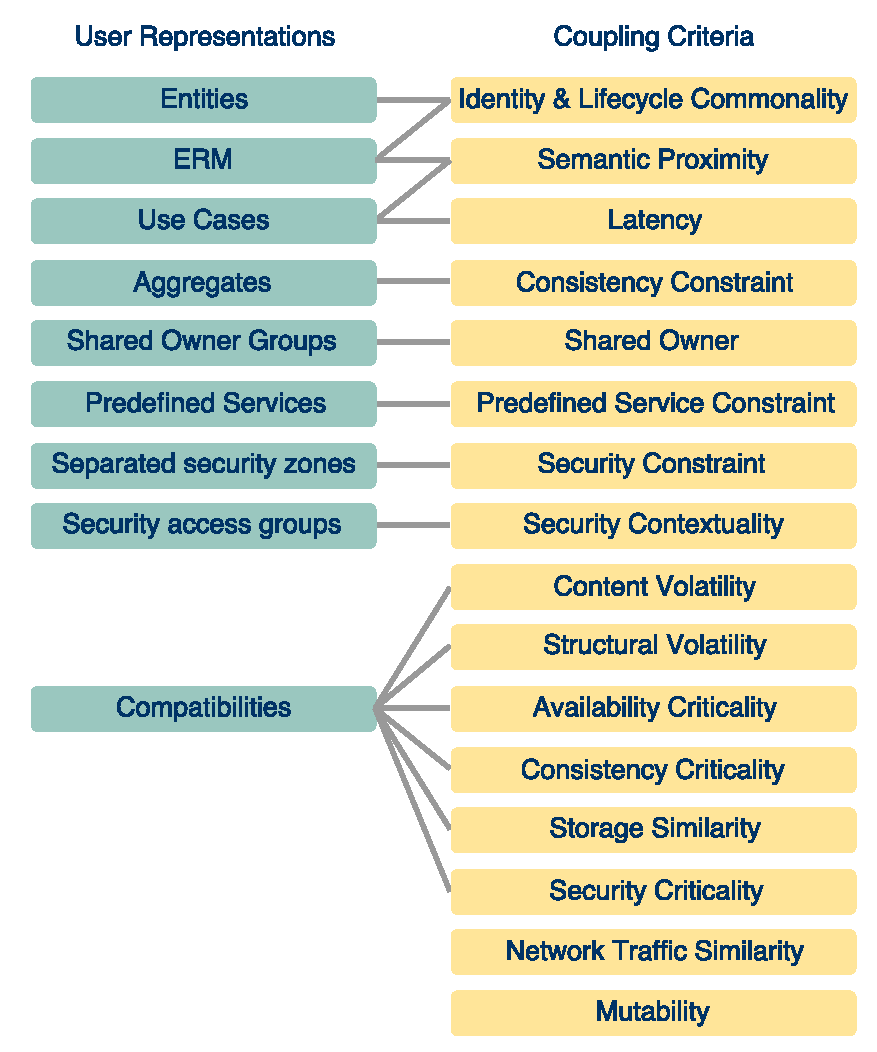
\includegraphics[scale=0.6]{diagrams/UserRep-CC.pdf}
		\caption{User representations and the related coupling criteria}
		\label{fig:userrep}
	\end{center}
\end{figure}

The technical format including \gls{JSON} schema files of all user representations is documented in detail on GitHub\cite{githubWiki}.

\section{Service Cut Analysis}

The Service Cutter offers an analysis mode. When activated, the relationships between services are visualized and the published language of the services is generated. Figure \ref{fig:service-dependency} outlines such a dependency: Nanoentities of Service A and D are read or written in a common use case. 

\begin{figure}[H]
	\centering{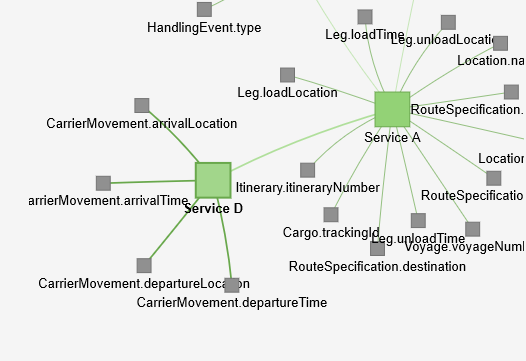
\includegraphics[scale=0.7]{images/screenshot-solver-analysis-example.png}}
	\caption{Service A and Service D share a use case.}
	\label{fig:service-dependency}
\end{figure}

The published language of Service D is visible in Figure \ref{fig:service-publang}.

\begin{figure}[H]
	\centering{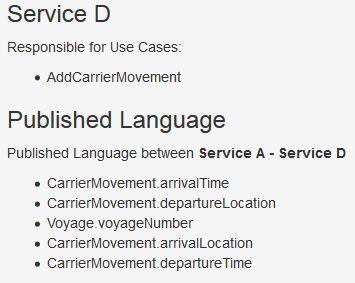
\includegraphics[scale=0.7]{images/screenshot-solver-analysis-service.png}}
	\caption{Use cases and published language of Service D}
	\label{fig:service-publang}
\end{figure}

\section{Usage Scenarios}

%TODO take from tutorial



%TODO rewrite
After introducing usage scenarios of the service cutter, the next chapter assesses the decomposition approach and the practicability of the Service Cutter

